\documentclass[lettersize,journal]{IEEEtran}
\usepackage{amsmath,amsfonts}
\usepackage{algorithmic}
\usepackage{algorithm}
\usepackage{array}
\usepackage[caption=false,font=normalsize,labelfont=sf,textfont=sf]{subfig}
\usepackage{textcomp}
\usepackage{stfloats}
\usepackage{url}
\usepackage{hyperref}
\usepackage{verbatim}
\usepackage{graphicx}
%\usepackage{cite}
\usepackage[numbers]{natbib}
\hyphenation{op-tical net-works semi-conduc-tor IEEE-Xplore}
% updated with editorial comments 8/9/2021

%%%%%%%%%%%%%%%%%%%%%%%%%%%%%%%%%%%%%%%%%%%%%%%%%%%%%%%
% URL line breaks in references
\def\UrlBreaks{\do\/\do-}

% todos
\usepackage{xcolor}
\newcommand{\todo}[1]{\textcolor{red}{TODO: #1}\PackageWarning{TODO:}{#1!}}
%%%%%%%%%%%%%%%%%%%%%%%%%%%%%%%%%%%%%%%%%%%%%%%%%%%%%%%

\begin{document}
	
	\title{Monitoring of Scientific Workflows}
	
	\author{Julian Legler, Marcin Ozimirski, Matthias Seiler
		% <-this % stops a space
		\thanks{This paper was produced by students at TU Berlin in the course ''Master Project: Distributed Systems''}% <-this % stops a space
		%\thanks{Manuscript received April 19, 2021; revised August 16, 2021.}
	}
	
	% The paper headers
	\markboth{PJ DS - Monitoring of Scientific Workflows}%
	{Shell \MakeLowercase{\textit{et al.}}: A Sample Article Using IEEEtran.cls for IEEE Journals}
	
	%\IEEEpubid{0000--0000/00\$00.00~\copyright~2021 IEEE}
	
	\maketitle
	
	\begin{abstract}
		
		The emergence of Scientific Workflow Management Systems (SWMS) allowed speeding up scientific progress in various fields. The main task of such systems is to represent and manage complex distributed scientific computations. They are designed to handle datasets and examine them in a programmatical way. The software can process given jobs effectively and provide results in a requested form. However, nowadays' scientific calculations can involve hundreds of stages, each integrating several models and data sources created by various groups. Because of their complexity, they require a significant amount of resources to be processed. Such projects are well suited to a cloud environment since it allows for scalability in the event of increased resource demand. In these situations, system monitoring software is essential because it provides a better understanding of how resources are utilized when consecutive tasks are being executed. It can help to decrease the costs by choosing the best suitable provider or adjusting parts of the code for a faster execution time. Unfortunately, the built-in monitoring features offered by the SWMS developers and cloud providers deliver only high-level metrics, such as CPU per task, which is not always enough for a detailed resource usage analysis. Therefore the implementation of software allowing for monitoring on a system process level stays on the shoulders of the end users. 
		
		% TODO: state our solution and result
		
	\end{abstract}
	
	\begin{IEEEkeywords}
		Scientific Workflow Management Systems, Monitoring, eBPF
	\end{IEEEkeywords}
	
	\section{Introduction}
	A scientific workflow management system (SWMS) is a commonly used software solution in the field of computational science. It can execute a series of calculations to examine (big) data sets in a structured and organized manner. Such computations are commonly called workflows consisting of tasks related to one another. The Management System is responsible for a transparent orchestration and execution of specified tasks, considering dependencies between them. The software allows for an efficient way to process and extract information from the examined data sets, leading to scientific advances in various fields such as biology, physics, and astronomy\cite{gil2007examiningchallengesscientific}. Yet, such workflows are often resource-intensive and require a distributed, dynamic, and scalable architecture to achieve meaningful results in a reasonable amount of time. The cloud and containerization paradigms offer several advantages when deploying these systems, such as accessibility, flexibility, and scalability \todo{source?}, which allow workflows to be deployed and executed dynamically. These characteristics are crucial, since a with a changing workflow during execution also comes different requirements regarding resources. This could for example depend on an input data set, the parallelism of computed tasks, and their level of complexity. The available resource pool can scale to adjust the computing resources throughout the workflow execution process. However, depending on the technological solutions offered by cloud services, hardware and software factors can vary significantly from one provider to another, which leads to different processing speeds, resource utilization, and error ratio\cite{aljamal2018comparativereviewhighperformance}. Built-in monitoring features provide information on the amount of time and resources needed for the computation of a particular task or resource utilization on the active virtual machines (containers). Unfortunately, for more intense calculations, like machine learning, data delivered by the built-in tools are often insufficient to provide enough information for deep analysis and detection of bottlenecks or finding opportunities for code optimization. In such scenarios, the more detailed (low-level) metrics available, the better conclusions can be drawn regarding the performance of the current solution. Producing exact information on the number of I/O operations, CPU load, or memory usage per system process allows for a more accurate analysis of executed workflows (or their tasks) and the infrastructure on which the calculations are performed. This would open doors for improving of the system architecture, hardware and code. However, the implementation of solutions capable of gathering such information or the extension of the already existing ones rests on the shoulders of the end users. This project intends to provide a solution allowing the collection of high- and low-level metrics, independently of underlying cloud technology and SWMS used for computational science. The following report is structured as follows \todo{}
	
	
	\section{Related Work}
	% TODO: previous research on SWMS, eBPF
	Due to the nature of high volume data, modern science is often conducted on high-performance computing infrastructures. In recent years, the complexity of both the complexity of scientific experiments, as well as that of its underlying infrastructure has grown tremendously, reaching the point where it becomes challenging to execute the workflows in a reliable and error-free way. On the scale at which such projects are carried out it is almost certain that software or infrastructure anomalies will occur, which makes the detection and diagnosis of system failures more challenging than ever before. In order to address such issues, \citeauthor{valerio2008capturingworkflowevent} created a prototype system monitoring the following \todo{} properties at any time during and after the execution of the workflow. The premise of the design is to enable the user to answer the following questions:
	
	\begin{itemize}
		\item What is the status of the workflow?
		\item Did the user make changes to the workflow before executing it?
		\item Why did it fail at a certain point?
		\item What was the execution context of the workflow directly before it failed?
		\item How many resources does it consume?
		\item How has each activity in the workflow performed (in the past)?
	\end{itemize}
	
	The ability to answer the aforementioned questions can be guaranteed by a system monitoring the general properties of the workflow and its slightest details. Therefore, this type of solution usually consists of various components that collect data at different layers, starting from the general parameters of the workflow through the infrastructure on which it is run, ending with individual processes responsible for performing calculations. In addition, the software must be able to map the relevant processes (which can be executed in a parallel and distributed manner) to the following machines and tasks and publish them in a readable form. Of course, all this makes sense only if one can assign a chronological order of these processes concerning the time domain. Furthermore, an environment in which such scenarios are executed also plays an important role. Regardless of whether the code is invoked in the operating system context or a virtualized container created for the task, it is often characterized by restrictive standards. Such standards fulfill the functions of stability and security and thus may not provide any or only limited opportunities for adjustment. However, without it, it may not be possible to access system values available to the system's kernel. 
	Fortunately, one does not have to develop everything from scratch as there are open technologies capable of solving a single or part of the listed conditions. \citeauthor{levin2020viperproberethinkingmicroservice} used Linux’s extended Berkeley Packet Filter (eBPF)\cite{ebpf} software for a collection of system metrics in the containerized environment and exposure of these to a specified endpoint. In a further step, he used Grafana\cite{grafana}, an observability framework, to present the collected information using programmable dashboards. This strategy allows the collection of data from various sources and then processing and presenting it in the form of histograms and graphs, as described by the user. It also reflects well the current trend for creating monitoring solutions. It is based on a combination of available platforms and software to collect and present data that are relevant to a carried-out project. For such approaches, it is not important what generates or where the data comes from, as long as it is published in a suitable format, which is most often JSON or some derivative of XML.
	
	\section{Background}
	% TODO: describe technologies we are using
	% k8s
	For the case of this project, the software is deployed to the Google Cloud Platform (GCP) \todo{ref} as a containerized cluster. Cloud technology ensures scalability, which is a must in the case of scientific workflows. During the execution of the pipeline, the number of resources needed for a smooth and timely execution can vary significantly. The resources provided by the cloud can scale together with the needs. In combination with container technology, one achieves a robust and scalable solution with access to a great pool of computational power. Kubernetes \todo{ref} is used for the orchestration of containerized workloads and services. It is an open-source platform, with a big community, decent documentation, and a great set of usage examples available online, became one of the most popular management tools for container environments.  
	
	% SWMS, Airflow
	Today exists a vast number of workflow management systems, ranging form general purpose ones like Apache Airflow \cite{airflow}, Nextflow \cite{nextflow} or Pegasus \cite{pegasus} to domain specific ones e.g. Taverna \cite{taverna} for bio-informatics and astronomy, Arvados \cite{arvados} for biomedical data and many more. Each of these naturally have their advantages and disadvantages over another, due to their design and architecture and thus resulting in different stages of maturity.\\
	We decided for Airflow, since it serves the general purpose, is widely used and one of the most mature SWMS. The workflow in Airflow is described in Directed Acyclic Graph (DAG), whose nodes consists of tasks that are executed. The edges represent the dependencies and therefore the execution order of these tasks. The description of the DAG is specified by the user in a Python script. Figure \ref{fig:aiflow:dag} shows DAG that runs tests in a Kubernetes environment \cite{airflowDag}.
	\begin{figure}[h]
		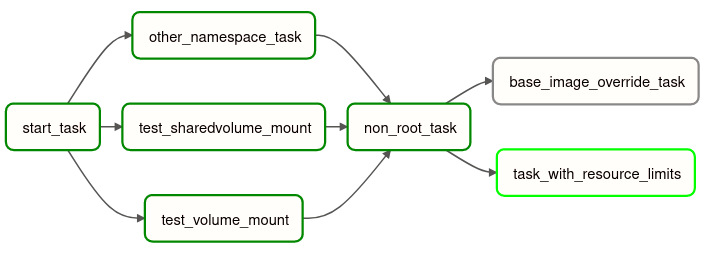
\includegraphics[width=\linewidth]{images/airflow-dag.png}
		\caption{Airflow DAG with five tasks successfully run (dark green), one running (light green) and one in queue (gray).}
		\label{fig:aiflow:dag}
	\end{figure}
	
	As depicted in Figure \ref{fig:aiflow:arch}, the basic architecture of Airflow consists of the following components: the \textit{User Interface}, that is served by the \textit{Webserver}, is the entry point for the user, and not only feature-rich, but also easy to use. At the heart of Airflow resides the \textit{Scheduler}, ''which handles both triggering scheduled workflows, and submitting Tasks''\cite{airflowArchitecture}. It therefore requires access to a \textit{DAG Directory}, in order to makes use of one of the provided \textit{Executor}s \cite{airflowExecutor}, that handle these tasks. The actual execution of tasks is performed by one or more \textit{Workers}. Finally, a \textit{Metadata Database} is ''used by the scheduler, executor and webserver to store state''\cite{airflowArchitecture}.
	\begin{figure}[h]
		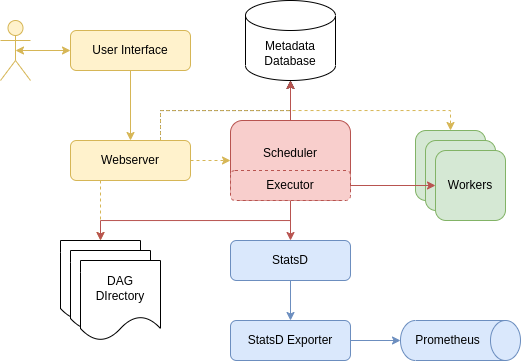
\includegraphics[width=\linewidth]{images/airflow-architecture.png}
		\caption{Airflow architecture \cite{airflowArchitecture}}
		\label{fig:aiflow:arch}
	\end{figure}
	
	Airflow provides built-in logging and monitoring \cite{airflowMonitoring}, whose monitoring stack relies on StatsD \cite{statsd}, that gather the internal metrics and exposes them to Prometheus \cite{prometheus}. While the are numerous metrics on DAG and task level, none of them consider metrics on lower levels \cite{airflowMetrics}.
	
	% Monitoring, eBPF
	With eBPF \cite{ebpf} however, it is possible to gather metrics directly from the Linux kernel. It extends the kernel without changing the kernel source code or loading kernel modules and has therefore unrestricted access to all hardware. These little programs get triggered by certain hook point (e.g. system calls, function entry/exit, network events) and can thus be attached to almost anywhere int kernel or user applications \cite{whatebpf}. 
	Figure \ref{fig:ebpf:steps} depicts the involved steps to attach an eBPF program: in order to use the program in the Linux kernel, it expects the program in the form of bytecode. With the \texttt{bpf} system call, the program will be loaded into kernel space, where it first has to be verified (that is actually safe to run) and secondly compiled to machine specific instructions. ''This makes eBPF programs run as efficiently as natively compiled kernel code or as code loaded as a kernel module'' \cite{whatebpf}.
	\begin{figure}[h]
		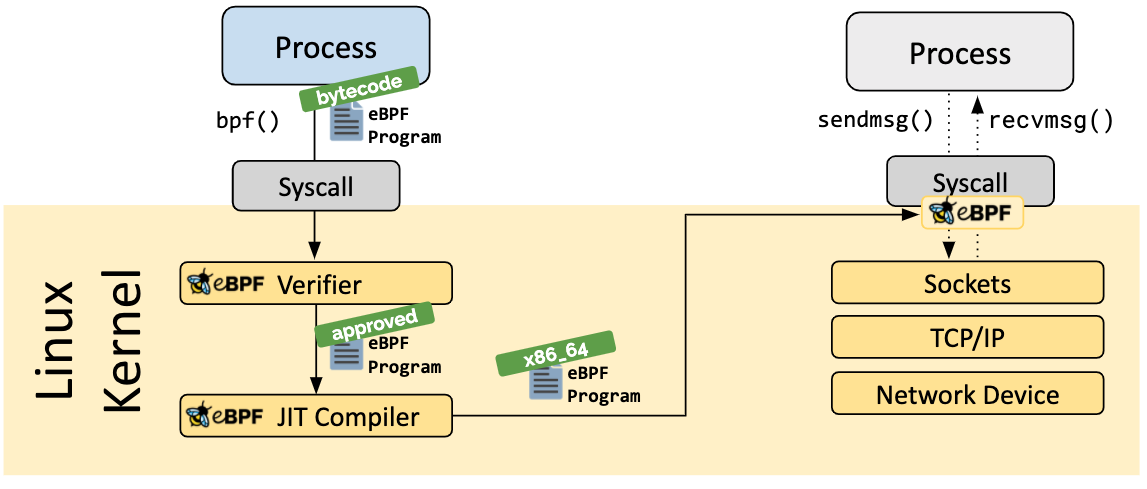
\includegraphics[width=\linewidth]{images/ebpf-steps.png}
		\caption{Steps to attach an eBPF program \cite{whatebpf}}
		\label{fig:ebpf:steps}
	\end{figure}
	In order to store collected information (e.g. in the form of metrics), eBPF leverages \textit{eBPF Maps} \cite{ebpfMaps}, that can be accessed not only from kernel, but also from user space.
	
	% Monitoring, Prometheus, Grafana
	The data from these eBPF maps can be exported to a more powerful monitoring systems such as Prometheus \cite{prometheus}, Graphite or InfluxDB, and  visualized with an analytics platform like Grafana or Kibana.
	
	
	\section{Approach}
	% TODO: how we implemented tech mentiones in background
	As mentioned in the previous section, we are going to build the monitoring solution on top of the Scientific Workflow Management System (SWMS) Apache Airflow. 
	
	\subsection{Architecture and Components of Apache Airflow}
	
	\begin{figure}[h]
		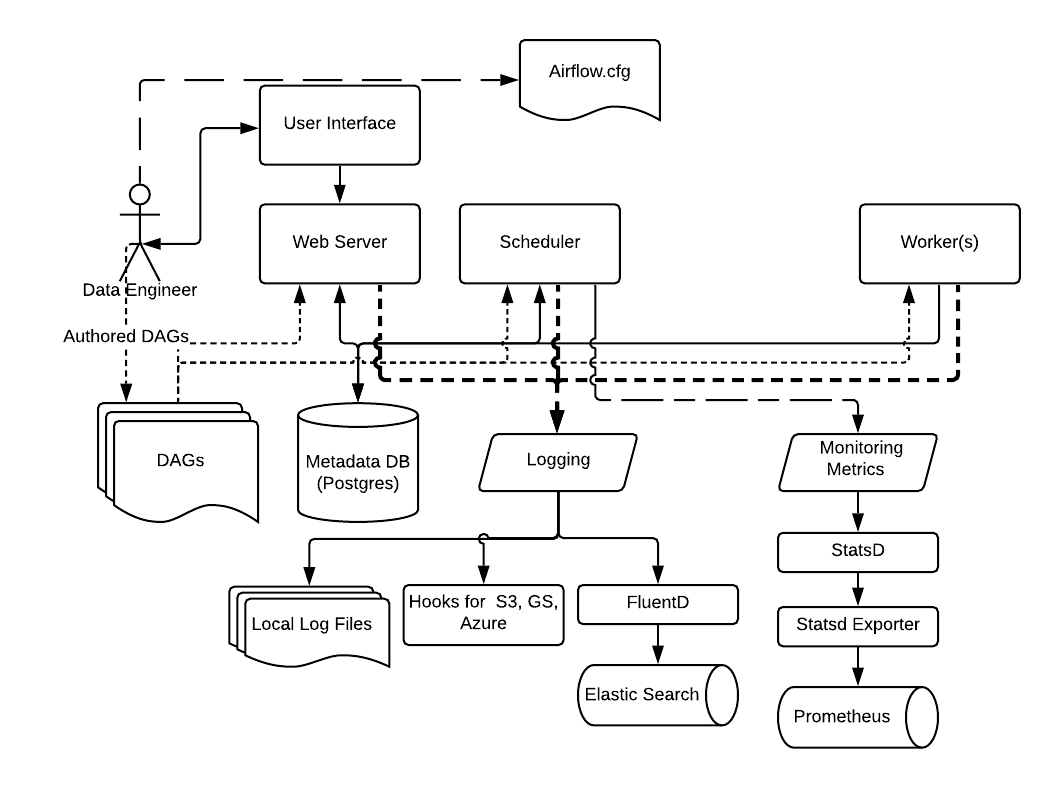
\includegraphics[width=\linewidth]{images/arch-diag-logging.png}
		\caption{Architecture of Apache Airflow extended Image}
		\label{fig:airflow_arch_logging}
	\end{figure}
	
	
	Apache Airflow consists of an Webserver running a GUI, a Database, an Scheduler and Executor, a Directory for DAGs, a Logging Component, Monitoring Component and one or multiple workers.
	
	The webserver is the graphical user interface for starting, stopping and monitoring currently running or already runned tasks.
	
	The database is for storing the current results, information and states of the system, jobs and tasks.
	
	The Scheduler is for triggering the execution of tasks and deciding in which order they get executed.
	
	The Executor has different operation modes, but in general, its work is to get the scheduled tasks actually running on workers.
	
	The Worker is the encapsulation of an actually running tasks.
	
	The Logging is done by using FluentD for log handing.
	
	For Monitoring, StatsD is used as the metric collector in the system. \cite{statsd} 
	It was originally developed by Etsy and works by creating buckets and filling them with values for the specific metric, after a predefined period the values will be aggregated and flushed to an endpoint for further handling. 
	
	
	\subsection{Deployment of Apache Airflow}
	Apache Airflow is a widely used and adopted SWMS and as such, there are many approaches for deployment. These include fully managed solutions like Google Cloud Composer, Amazon Managed Workflows for Apache Airflow and astronomer.io. Using such services comes with the advantage of an easy and fast deployment. The downside is, that you may lack some flexibility and access to more granular and in depth functionalities and access. An Apache Airflow deployed by such services can often just be treated as a black box system. This approach may block some needed functionalities and access to the raw resources required to collect metrics at the level of granularity we try to achieve.
	
	On the other side of the Deployment complexity are the deployment strategies that involves deploying or sometimes even compiling the needed components yourself on bare-metal servers. For this, the database and logging systems have to be correctly installed before. At the same time, machines have to be configured to build a cluster and then Apache Airflow is installed and run on all the machines. This could also be combined by deploying Kubernetes in the first place, and then using Kubernetes orchestration technologies to run all the needed services in the cluster. This deployment strategy comes with the advantage of fine and granular access to all system resources, but the downside is the overhead of managing everything by yourself. 
	
	A deployment strategy is picked, that combines the two above. Google Cloud Platform (GCP) is used as the provider for the needed computation power provided by their different cloud services. GCP provides managed resources and guarantees an easy-to-use process of deploying the needed infrastructure. With the Google Kubernetes Engine (GKE) it even provides a managed Kubernetes deployment. Using this, the services no longer have to be installed on the individual machines, they can rather be just send to Kubernetes and then Kubernetes orchestrates the needed services and deploy them on the available infrastructure. At the same time, one has full access to all the underlying components, like the virtual machines Kubernetes and the Apache Airflow services running on. This combines the granular access to all resources, and the ease of using a managed service.
	
	GKE is configured to create three nodes of the type e2-standard-4 which consist of 4 vCPUs and 16 GB RAM. \cite{gcpMachineType}
	For the deployment of Apache Airflow on top of Kubernetes the official Apache Airflow Helm Chart is used. \cite{airflowHelmChart} Using a Helm Chart is a good way to reduce further complexity by using a pre-defined, out of the box running, Apache Airflow configuration. 
	
	The original Helm Chart was altered in the following ways to deal with our requirements.
	\subsubsection{Executor — \todo{we are missing a chapter that explains how apache airflow is build internally?}}
	The Executor is the service, that takes the scheduled tasks and takes all needed steps to get them executed by the worker.
	
	“An Airflow installation generally consists of [...] An executor, which handles running tasks. In the default Airflow installation, this runs everything inside the scheduler, but most production-suitable executors actually push task execution out to workers.”
	“Airflow sends out Tasks to run on Workers as space becomes available, so there’s no guarantee all the tasks in your DAG will run on the same worker or the same machine.”
	
	
	\begin{figure}[h]
		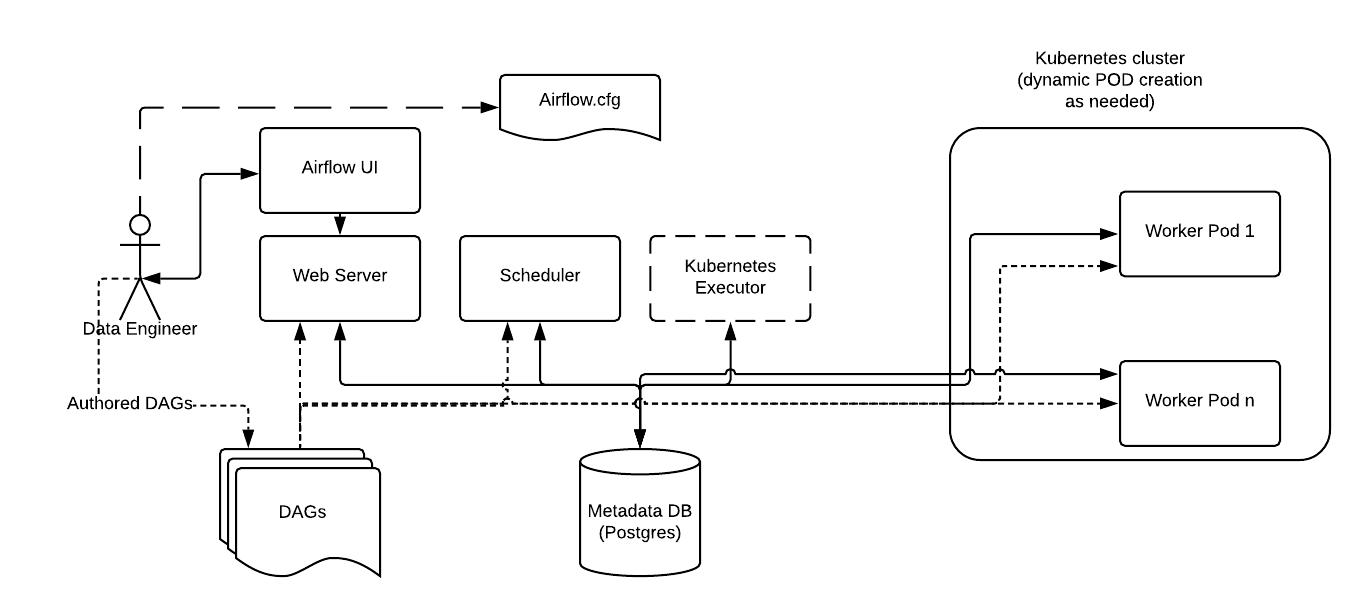
\includegraphics[width=\linewidth]{images/arch-diag-kubernetes.png}
		\caption{Kubernetes Executor image}
		\label{fig:airflow_arch_kubernetes}
	\end{figure}
	
	
	There are multiple different Apache Airflow Executors with different approaches on how to handle the execution of tasks. We compared the default Celery Executor to the Kuberentes Executor:
	
	Celery Executor is adding a Queue to the deployment. On all available nodes, a worker will be deployed. The workers just endlessly fetching new jobs from the queue and working on them. 
	
	Kubernetes Executor is changing the behavior in the way, that no longer each node has one worker, but rather for each job there is one worker which is terminated when the job is finished.
	
	The huge advantage of the Kubernetes Executor is, that this executor is using the labeling capabilities of Kubernetes. The Kubernetes Executor is very communicative in the worker name and metadata, which makes it easy to collect all this information without accessing the machine.
	
	\subsubsection{StatsD}
	StatsD is the Logging and Metrics service used by Apache Airflow. To get the metrics compatible to Prometheus, a mapping is configured, so that the values can will be correctly interpreted by Prometheus.
	
	\subsubsection{Webserver, Worker, Environment}
	Here are just minor changes, so that the access to the web server can be easily done, the right amount of worker nodes get configured and some environment parameters are changed to deal with some encountered issues.
	
	\subsubsection{Prometheus and Grafana}
	For the monitoring stack Prometheus and Grafana are used. To get them working, the following changes are done.
	
	Apache Airflows StatsD Exporter is added as a scraping target
	Every Endpoint is scraped for ebpf values
	
	kube-state-metrics now send all Labels and Annotations from all pods in all namespaces and not stripping them away before sending them to Prometheus.
	
	Because of the mapping already done via the StatsD exporter, the metrics are parsable and interpretable as normal Prometheus metrics.
	
	\subsection{eBPF}
	The used eBPF exporter is a fork of the eBPF exporter by Cloudflare \cite{ebpfCloudflare} and is extended with a previously not accepted pull request that implements a sample for using eBPF with Kubernetes. \cite{ebpfPull75} Additionally, existing sample BPF code was added from the BPF Compiler Collection (BCC) samples. \cite{bcc}
	The eBPF exporter is available on Docker Hub and is automatically pulled when a new node is created. It runs on every node in the Kubernetes Cluster. 
	\todo{Problem Docker API expired because DockerD no longer supported in Kubernetes. (\url{https://kubernetes.io/blog/2020/12/02/dont-panic-kubernetes-and-docker/}) ContainerD is the replacement but the ContainerD API is terrible and not usable because the lack of documentation. We had to switch to Kubernetes API but then had to also deal with authentication mechanics because it was operating on the cluster, not on itself.}
	
	
	To do all this automatically, an own Helm Chart is created with all the needed configurations. 
	…
	
	
	\section{Discussion}
	% TODO: results and challenges
	\subsection{eBPF Challenges}
	\subsection{Nextflow Challenges}
	
	\section{Conclusion}
	
\includegraphics[width=\linewidth]{images/placeholder.jpg}
	\todo{remove placehodler}
	
	\section*{Acknowledgments}
	We thank our supervisor Sören Becker for his enormous support and patience. 
	
	% References
	\bibliography{bib}
	\bibliographystyle{IEEEtranN}
	
\end{document}